\documentclass[11pt]{article}
\usepackage[french]{babel}
\usepackage[T1]{fontenc}
\usepackage{fontspec}
\usepackage[utf8]{inputenc}
\usepackage{url}
\usepackage{eurosym}
\usepackage{pdfpages}
\usepackage{ulem} % to use a strikeout/strikethrough font
\usepackage{color}
\newcommand{\fs}[1]{\textcolor{red}{\sout{#1}}}
\newcommand{\f}[1]{\textcolor{blue}{#1}}
\usepackage{graphicx} % Inclure des images
\usepackage{multicol} % Multi-colonnes


\usepackage[autolanguage, np]{numprint} % écriture des virgules
\usepackage[top=3cm,right=2cm,bottom=2cm,left=2cm]{geometry}


\usepackage[autolanguage, np]{numprint} % écriture des virgules

\title{HAUM}
\author{Assemblées Générales Ordinaire \& Extraordinaire}
\date{14 Juillet 2022}

\begin{document}
\maketitle

\section*{Convocation}

Madame, Monsieur,

L'association HAUM vous convoque à ses Assemblées Générales Ordinaire \& Extraordinaire qui se tiendront le :

\begin{center}
{\Large 14 Juillet 2022 à 15h00}\\
à Le Mans Innovation, \\57 Bd Demorieux au 2\textsuperscript{ème} étage, \\72 100 Le Mans
\end{center}

En cas d'impossibilité, vous pouvez vous faire représenter si vous le souhaitez (2 procurations maximum par personne présente, Statuts, art. 6).

\newpage

\hrule
\vspace{.6cm}
\begin{center}
\Large\bfseries Assemblée Générale Ordinaire
\end{center}
\vspace{.3cm}
\hrule

\vspace{1.5cm}

\section*{Déroulement}

\begin{enumerate}
    \item Présentation de l'association
    \item Rapport moral
        \begin{enumerate}
            \item Bilan
            \item Objectifs
            \item Questions
        \end{enumerate}
    \item Rapport financier
        \begin{enumerate}
						\item En images
            \item Bilan \& Objectifs
            \item Questions
        \end{enumerate}
    \item Motions et vote
    \item Élection du nouveau bureau
    \item Questions diverses
\end{enumerate}

\section{Présentation de l'association}

\section{Rapport Moral}

\subsection{Vie de l'association}

Le nombre de membres de l'association à jour de cotisation a diminué au cours de l'épidémie de Covid-19 toutefois on notera que plusieurs entreprises ont exprimé la volonté d'adhérer au niveau institutionnel. En particulier, une entreprise est entrée en contact avec l'association pour pouvoir payer une adhésion globale pour permettre à ses employés de profiter de l'accès au local et aux outils/machines. Cette piste est à explorer dans les prochaines années.

À compter de mai 2022, le HAUM se sépare progressivement de sa mailing-list au profit d'un forum 
disponible à l'adresse \url{https://forum.haum.org}. Les convocations aux prochaines Assemblées Générales passeront par ce biais dans le futur.

\subsection{Bilan}

\subsubsection{Le Mans Innovation}

Suite au déménagement en 2017, le HAUM a largement investi le nouveau local. L'association dispose d'un atelier propre et d'un atelier sale dont la tenue globale laisse aujourd'hui à désirer. Suite à l'intégration au sein du local de plusieurs entreprises présentes sur le plateau (Chaînes de Pluie, Laboa, Furion Motorcycles), une place de plus en plus importante leur est concédée. Les entreprises en question n'utilisent plus les surfaces de fabrication et utilisent aujourd'hui cet espace comme stockage.

Grâce à un don de l'Université du Mans, le local s'est équipé en mobilier, notamment en tables et établis et des discussions sont actuellement en cours avec Le Mans Innovation pour installer une zone de stockage sur étagères. 

Il est important de mettre en place un roulement pour le rangement du HAUM et maintenir le local dans un état utilisable.

\subsubsection{Évènements}

Depuis 2017, Le HAUM a participé à de nombreux évènements et proposé autant de
projets innovants. Voici les plus marquants.

\paragraph{Teriaki} Le festival Teriaki s'est, comme à l'accoutumée, déroulé à la fin
août. Le HAUM était présent avec une nouvelle invention nommée GyroPong. Basé sur la détection de codes Aruco par une caméra située en hauteur du terrain de jeu, il s'agit d'un pong en réalité augmentée.

\paragraph{24h du code} Le HAUM a réitéré sa participation aux \textit{24h du code} en proposant
une nouvelle épreuve. Le sujet, répondant au nom de gHaumCube64, portait sur la compréhension du protocole SACN, utilisé dans le milieu du spectacle pour le pilotage de divers éclairages et autres machines à fumée.
Le HAUM avait pour cela proposé un cube en trois dimensions, composés de 64 petites lumières nommées tål, et pilotable via le protocole SACN. Le HAUM a proposé un sujet chaque année depuis 2017.

\paragraph{Le Mans Sonore} La structure issue des 24h du code 2021 a été réutilisé pour proposer un élément scénographique dans le cadre de Le Mans Sonore 2022.

\subsubsection{Projets et axes}

Il y a plusieurs projets en cours. Au niveau collectif (pour des projets qui occupent
quelques personnes) on a aujourd'hui:

\begin{description}
	\item[Photographie] Sténopé, stéréo-photographie, etc\ldots
	\item[Lumière] Plusieurs projets également : scratch holograms, light painting, moirés, Tål
	\item[IdiHAUM\footnotemark]\footnotetext{Nom non définitif} Solution de contrôle d'accès
\end{description}

Les réunions "projets" qui avaient été proposées et instaurées lors de la dernière année
ont été plutôt bien suivies et utiles au début de l'exercice et ont complètement disparu
pendant l'été. Elle permettaient à tous de s'informer des projets en cours régulièrement
et une solution de remplacement est peut être à chercher.

\subsection{Matériel disponible}

Le HAUM dispose actuellement du matériel suivant (entre autres):

\begin{description}
    \item Une découpeuse laser (Pret de Le Mans Innovation)
    \item Une imprimante 3D (Pret de Le Mans Innovation)
    \item Une découpeuse vinyle Caméo (plotter de découpe)
    \item Outils pour l'électronique (dont plusieurs fers à souder donnés par ST Microelectronics)
    \item Outillage électroportatif et manuel
    \item Fraiseuse CNC 3 axes de table
    \item La majorité des projets passés
\end{description}

\subsection{Objectifs}

Lors de l'année 2019, de nombreux projets ont pu être menés à terme, malgré une baisse de la
fréquentation de l'association. S'en est suivi une crise sanitaire saupoudrée de plusieurs 
confinements pour finir d'abattre la fréquentation du lieu. Des solutions alternatives ont 
malgré tout pu être trouvées (notamment la mise en place de réunion par visio), mais cela 
n'a pas suffit pour maintenir la fréquentation a un niveau suffisant.

Suite à la réouverture de nos droits de déplacement et d'ouverture du local, nous avons pu
noter un regain dans la fréquentation, ainsi que l'arrivée de nombreuses nouvelles personnes
qui souhaitaient trouver un lieu de bidouille et de convivialité.

Quelques déplacements et projets ont pu être repris ‑ on pense notamment à Teriaki, ou les 
24h du code ‑ mais il est clair qu'il est nécessaire de «relancer la machine» pour pouvoir 
attirer de nouveaux membres et ainsi créer une dynamique nouvelle dans les futurs projets.



\section{Rapport financier}

\begin{center}
%\begin{multicols}{2}
%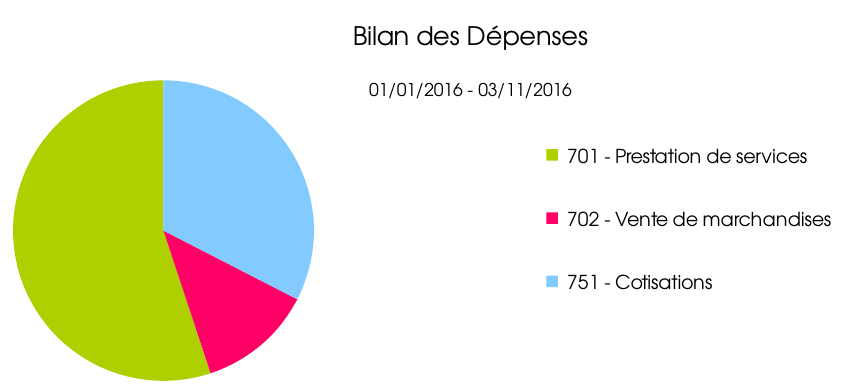
\includegraphics[width=8cm]{1DossierAGRecettes.png}

% 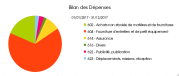
\includegraphics[width=8cm]{2DossierAGDepenses2017.png}
%\end{multicols}



\begin{multicols}{2}
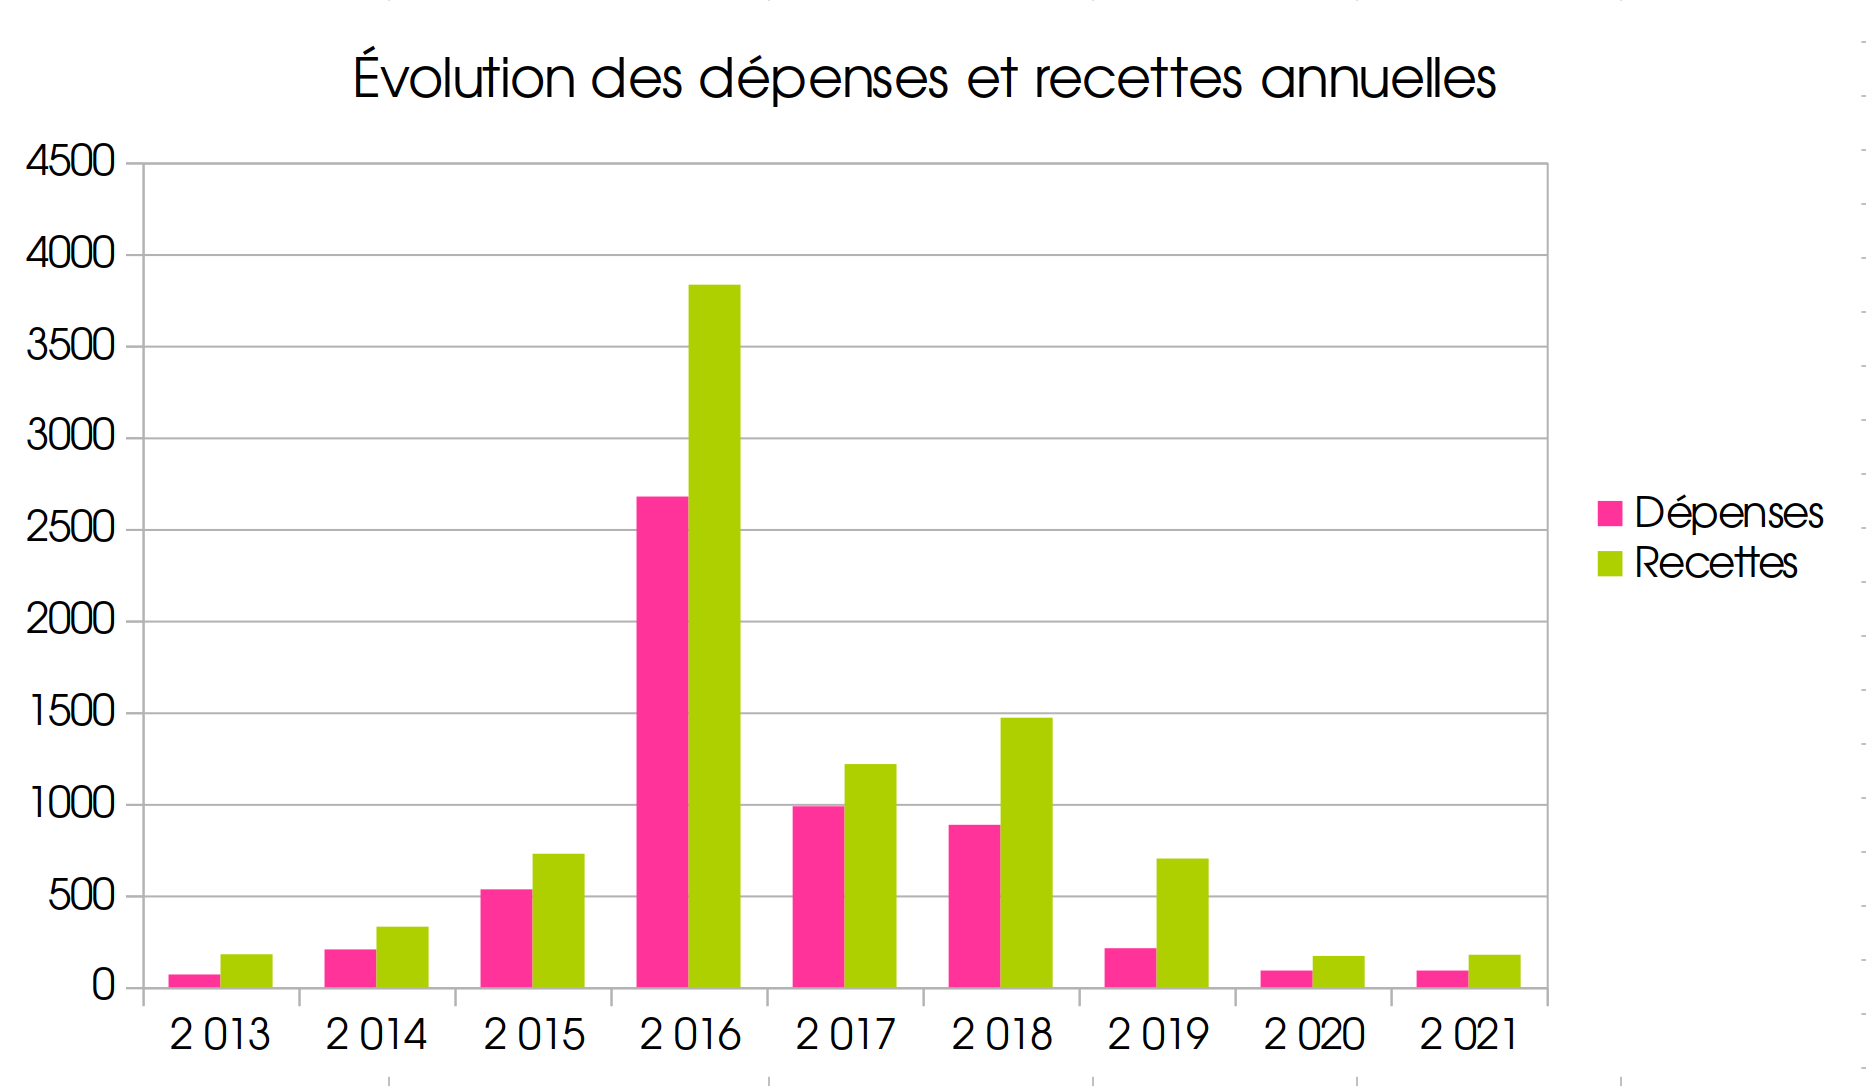
\includegraphics[width=8cm]{3DossierAGGeneral2021.png}

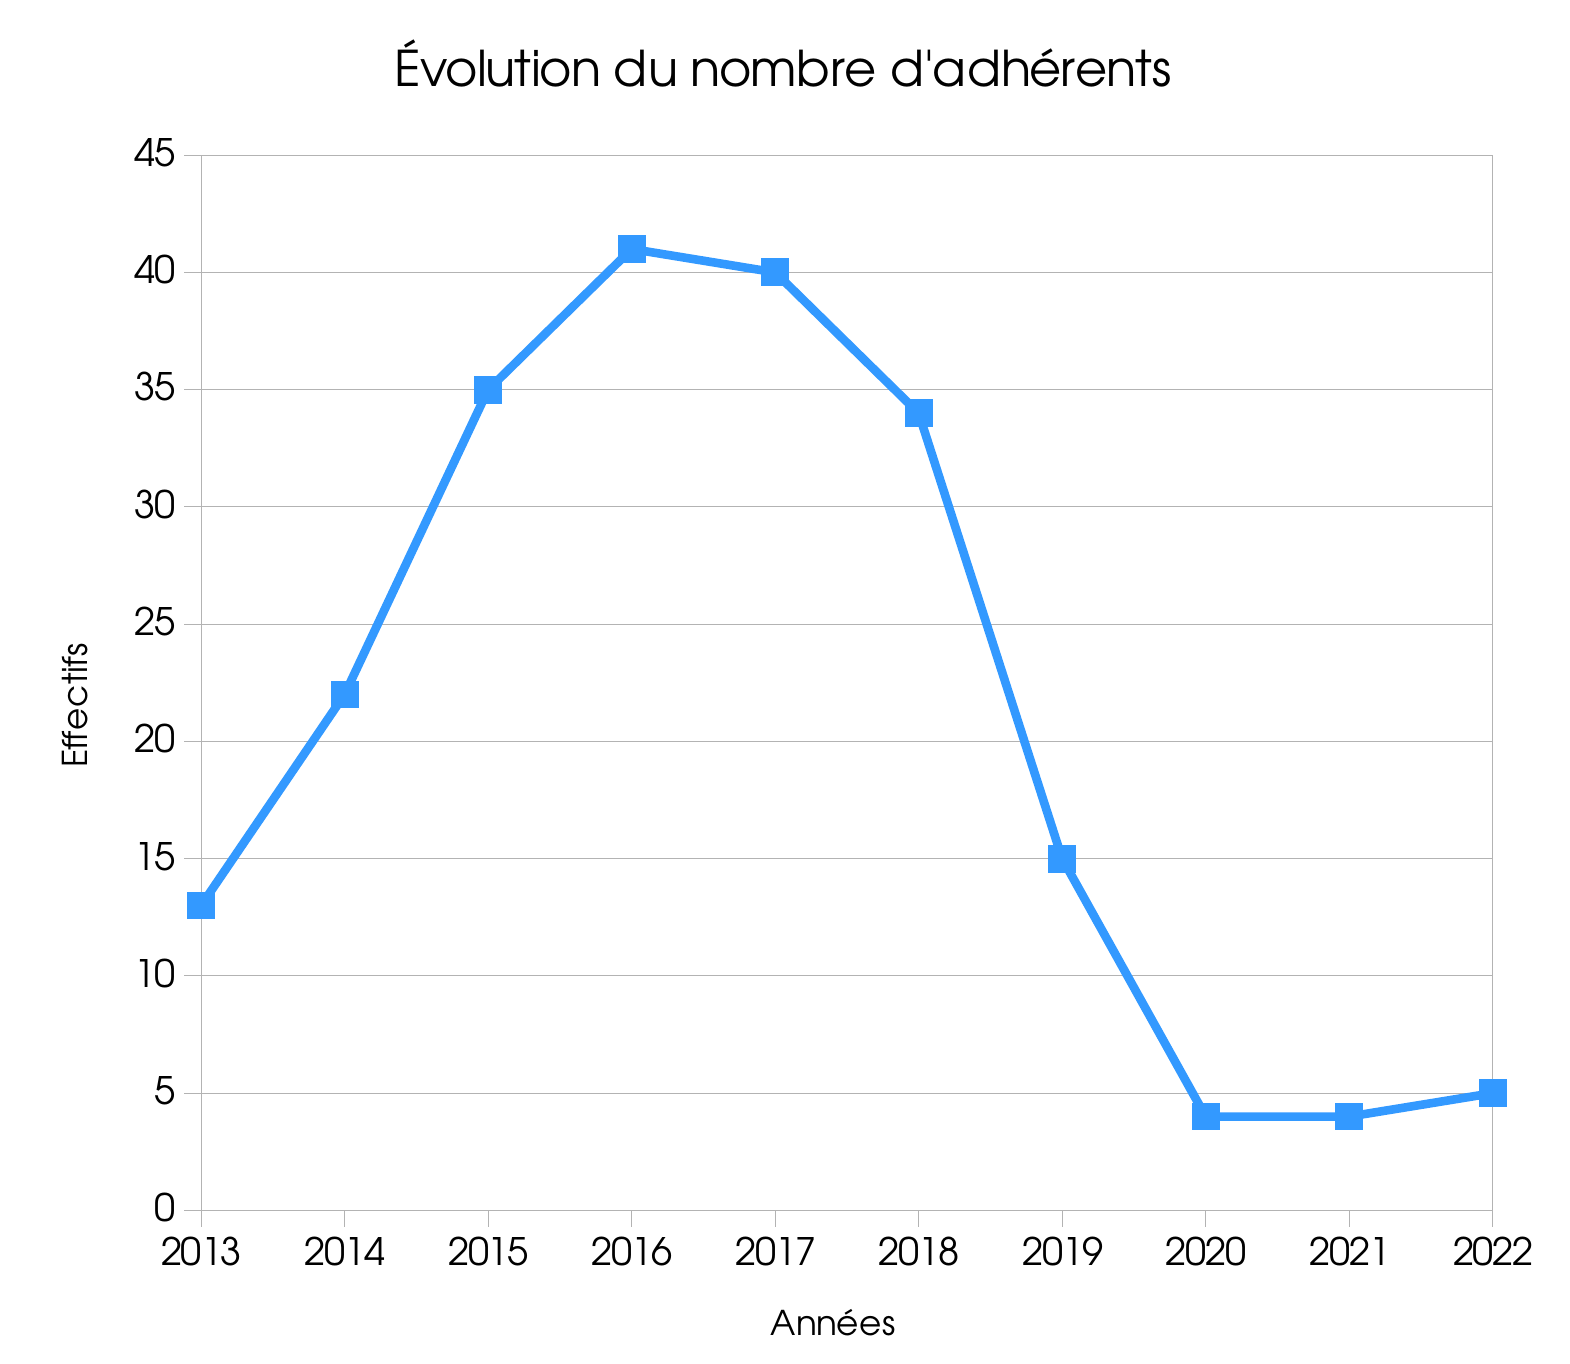
\includegraphics[width=8cm]{4DossierAGAdherents2021.png}
\end{multicols}
\end{center}

\section{Motions}

\subsection{Adhésion des membres partenaires}

Pour simplifier les adhésions de personnes morales, il est proposé de modifier 
les modalités d'adhésion des membres partenaires comme suit:

\begin{quote}
\itshape
\textbf{Membre partenaire}
Accessible uniquement aux personnes morales, via une cotisation annuelle.
Les membres partenaires peuvent voter pour une voix en assemblée
générale ordinaire et participer aux convocations du bureau par les membres.

Les plages de cotisation sont fixées comme suit:
\begin{itemize}
    \item Jusqu'à 5 employés : 250\officialeuro
    \item Jusqu'à 15 employés : 750\officialeuro
    \item Jusqu'à 30 employés : 1500\officialeuro
    \item Jusqu'à 60 employés : 3000\officialeuro
    \item Plus de 60 employés : 5000\officialeuro
\end{itemize}

Une négociation au cas par cas peut être envisagée avec le bureau de l'association.
\end{quote}

\subsection{Suppression de l'article 9}

Le bureau propose la suppression de l'offre de services aux extérieurs via la révocation de l'article 9 du règlement intérieur.

\section{Questions Diverses}

\newpage

\hrule
\vspace{.3cm}
\begin{center}
\Large\bfseries Assemblée Générale Extraordinaire
\end{center}
\vspace{.3cm}
\hrule

\vspace{1.5cm}

\section*{Déroulement}

\begin{enumerate}
    \item Appel et annonce des procurations
    \item Modification du siège social
	\item Modification des modalité d’organisation des assemblées
\end{enumerate}

\setcounter{section}{1}
\section{Modification du siège social}

L'article 3 des statuts est à modifier comme suit:

\begin{quote}
\itshape
Le siège social est fixé au 57 boulevard Demorieux, 72 100 Le Mans.
\end{quote}

\section{Modification des modalité d'organisation des assemblées}

L'article 9 est modifié comme suit :

\begin{quote}
\itshape
L’assemblée générale ordinaire comprend les membres actifs de l’association.

Elle se réunit au moins une fois par année calendaire, à une date fixée par le bureau.

Quinze jours au plus tard avant la date fixée, les membres actifs sont convoqués via le mode de communication électronique privilégié de l'association.

Les membres actifs dans l’impossibilité de se rendre à l’assemblée générale peuvent donner procuration à un autre membre actif de l’association pour les représenter selon les modalités précisées dans le règlement intérieur.

L’assemblée délibère sur tous les points inscrits à l’ordre du jour. Les décisions sont prises selon les
modalités précisées dans le règlement intérieur.
\end{quote}

\section*{Clotûre}

\newpage

\clearpage
\thispagestyle{empty}
\topskip0pt
\vspace*{\fill}
\begin{center}
\hrule
\vspace{.3cm}
\Huge\bfseries Annexes
\vspace{.3cm}
\hrule
\vspace{2cm}
\Large
\noindent Bilan Général 2013 -- 2021
\end{center}
\vspace*{\fill}

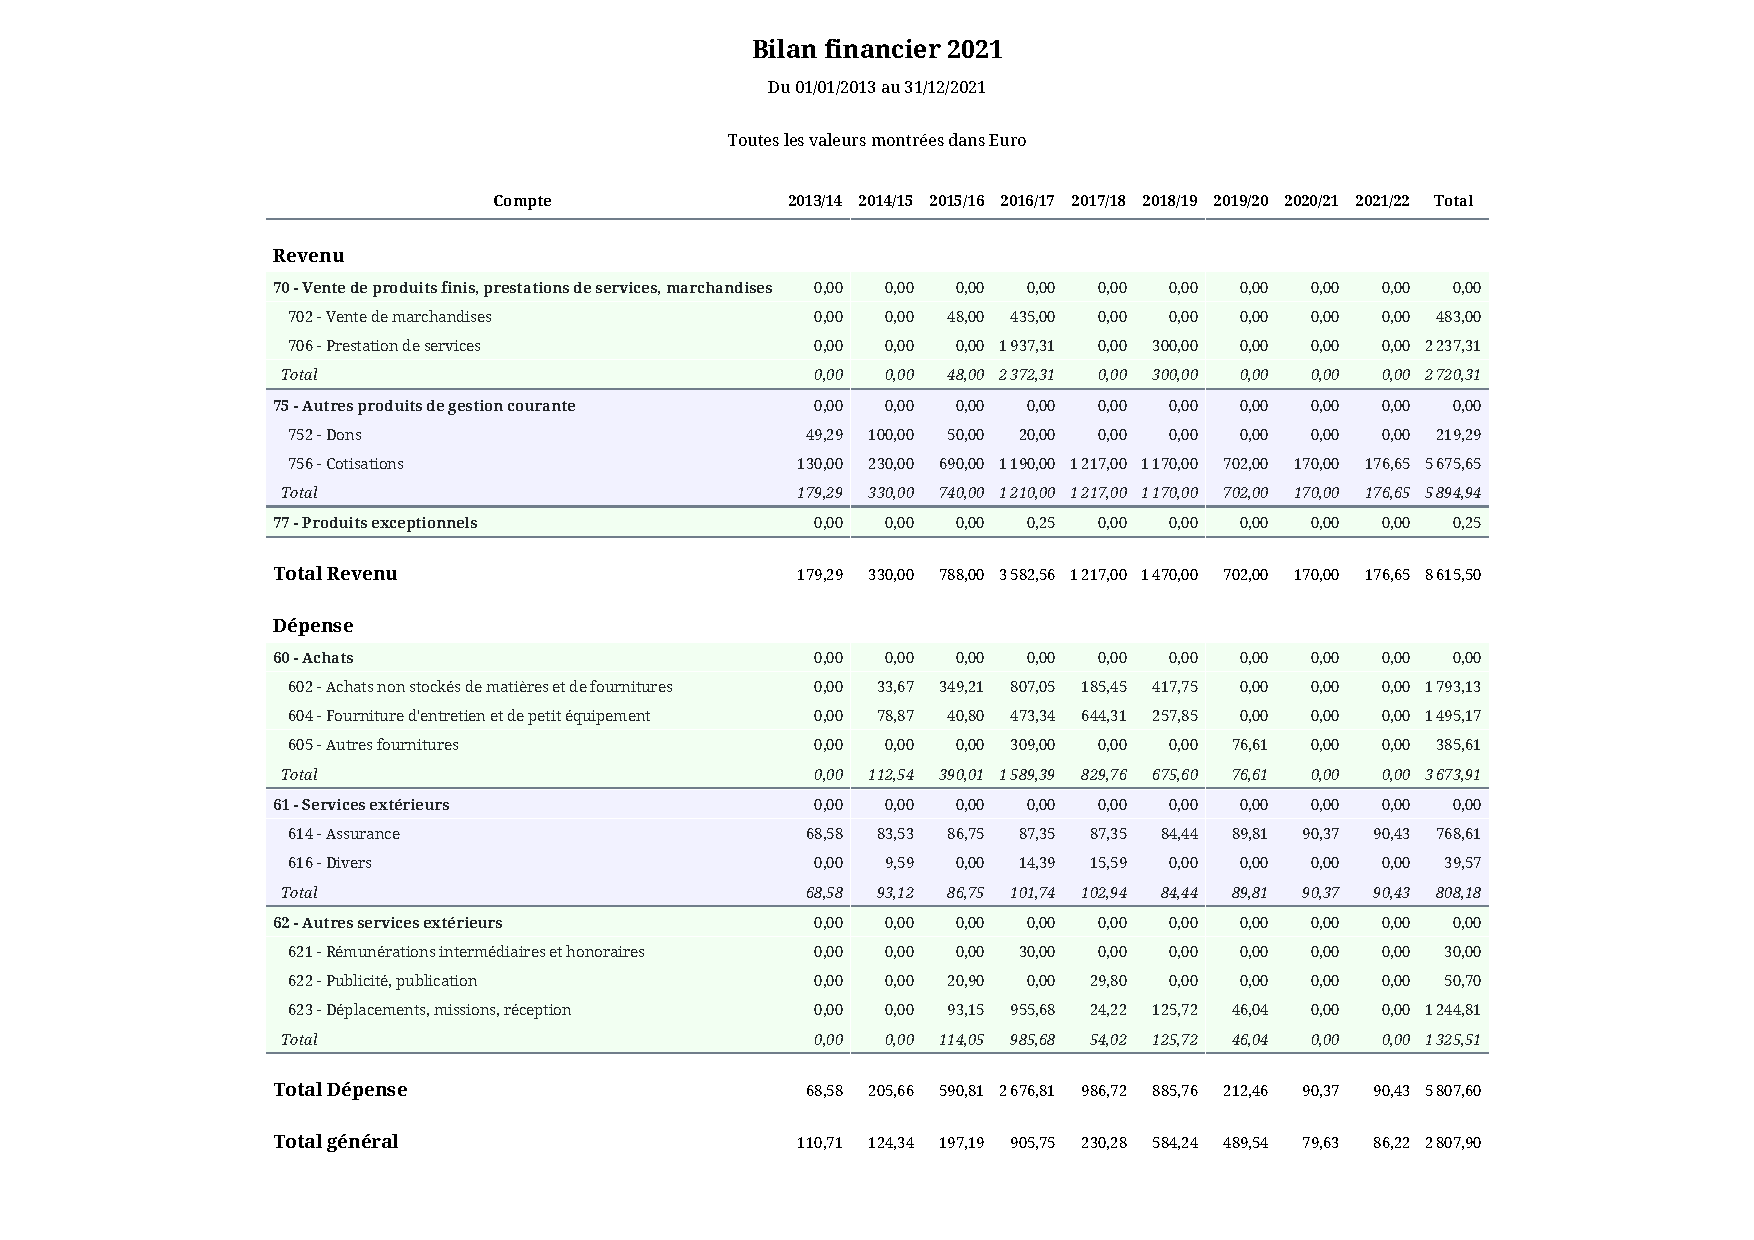
\includepdf[pages=-]{BilanGénéral2021.pdf}

\end{document}

% vim: set spelllang=fr:

